\documentclass[conference]{IEEEtran}
\IEEEoverridecommandlockouts

\usepackage{cite}
\usepackage{amsmath,amssymb,amsfonts}
\usepackage{graphicx}
\usepackage{textcomp}
\usepackage{xcolor}
\usepackage{booktabs}
\usepackage{array}
\usepackage{tabularx}
\usepackage{microtype}        % fixes most line-breaking issues
\usepackage{hyperref}
\hbadness=10000               % suppress underfull hbox warnings in narrow table cells
\usepackage{tikz}
\usetikzlibrary{arrows,positioning,shapes.geometric,fit,backgrounds,calc}
\hypersetup{colorlinks=false, breaklinks=true}

% Allow slightly looser line-breaking globally to kill underfull hboxes
\setlength{\emergencystretch}{2em}

%% ── TikZ style definitions ────────────────────────────────────────────────
\tikzset{
  device/.style={
    rectangle, rounded corners=3pt, draw=black!70, fill=gray!12,
    minimum width=1.4cm, minimum height=0.65cm,
    font=\scriptsize\sffamily, align=center, line width=0.5pt
  },
  master/.style={
    rectangle, rounded corners=3pt, draw=black!80, fill=blue!15,
    minimum width=1.5cm, minimum height=0.85cm,
    font=\scriptsize\sffamily\bfseries, align=center, line width=0.7pt
  },
  controller/.style={
    rectangle, rounded corners=3pt, draw=black!80, fill=orange!20,
    minimum width=1.5cm, minimum height=0.85cm,
    font=\scriptsize\sffamily\bfseries, align=center, line width=0.7pt
  },
  cloud/.style={
    rectangle, rounded corners=3pt, draw=black!60, fill=green!12,
    minimum width=1.5cm, minimum height=0.65cm,
    font=\scriptsize\sffamily, align=center, line width=0.5pt
  },
  iolink/.style={->, >=stealth, line width=0.8pt, color=blue!60},
  ethernet/.style={->, >=stealth, line width=0.8pt, color=orange!70, dashed},
  flow/.style={->, >=stealth, line width=1pt, color=black!70},
  dataflow/.style={->, >=stealth, line width=0.8pt, color=blue!60, dashed},
  acyclic/.style={->, >=stealth, line width=0.8pt, color=red!60, densely dotted},
  procbox/.style={
    rectangle, rounded corners=3pt, draw=black!60, fill=gray!10,
    minimum width=1.7cm, minimum height=0.7cm,
    font=\scriptsize\sffamily, align=center, line width=0.5pt
  },
  decision/.style={
    diamond, draw=black!70, fill=yellow!20,
    minimum width=1.3cm, minimum height=0.85cm,
    font=\scriptsize\sffamily, align=center, line width=0.5pt,
    inner sep=1pt
  },
}

\begin{document}

\title{IO-Link Communication Standard: Architecture,\\
Smart-Device Functions}

\author{
  \IEEEauthorblockN{Md Wasib Kamal Nirjon}
  \IEEEauthorblockA{
    \textit{Electronic Engineering}\\
    \textit{Hamm-Lippstadt University of Applied Sciences}\\
    Lippstadt, Germany\\
    md-wasib-kamal.nirjon@stud.hshl.de
  }
  \and
  \IEEEauthorblockN{Md Ratul Ahmed Alvi}
  \IEEEauthorblockA{
    \textit{Electronic Engineering}\\
    \textit{Hamm-Lippstadt University of Applied Sciences}\\
    Lippstadt, Germany\\
    md-ratul-ahmed.alvi@stud.hshl.de
  }
}

\maketitle

\begin{abstract}
Modern automation systems require more than a simple on/off signal from
a field device. Maintenance teams also need identification, parameter,
status, and diagnostic information that conventional wiring cannot
provide. This paper examines the IO-Link communication standard,
standardized as the Single-drop Digital Communication Interface in
IEC~61131-9. We explain how the physical connection, master-device
structure, cyclic and acyclic data channels, and the IO Device
Description (IODD) work together. We then evaluate IO-Link against the
communication requirements of a small automated packaging and sorting
cell. The comparison with conventional binary and 4--20\,mA interfaces
shows that IO-Link fits well at the last-meter connection of intelligent
sensors and actuators. It improves transparency and simplifies device
replacement, but does not replace controller-level Industrial Ethernet.
Its main limitations are the 20\,m cable restriction, modest bandwidth,
master cost, and the need for higher-level security measures not
included in the base protocol.
\end{abstract}

\begin{IEEEkeywords}
IO-Link, IEC~61131-9, industrial communication, smart sensor,
diagnostics, parameterization, Industry~4.0
\end{IEEEkeywords}

%% ---------------------------------------------------------------
\section{Introduction}
\label{sec:intro}
%% ---------------------------------------------------------------

Industrial machines depend on sensors and actuators that sit close to
the physical process. A photoelectric sensor detects a bottle on a
conveyor, a pressure sensor monitors a pneumatic line, and a valve
changes the flow. For a long time these devices were wired directly to
a programmable logic controller (PLC) using binary 24\,V signals or
4--20\,mA analog loops. This works well for simple cases, but it only
brings the raw measurement into the controller. Information about
device health, internal temperature, contamination, or configuration
stays locked inside the device and is invisible to the system.

This becomes a real problem when production changes frequently. If a
packaging line switches between bottle sizes, a technician must visit
each sensor and adjust the threshold manually. When a sensor fails, the
replacement must be configured from a datasheet. Both situations cost
time and introduce human error.

IO-Link was developed to solve exactly this problem at the sensor and
actuator level. IEC~61131-9 defines it as a point-to-point digital
interface for exchanging process values, parameters, identity, and
diagnostics with a smart field device~\cite{iec61131}. Importantly,
IO-Link is not a fieldbus. It does not compete with PROFINET, EtherCAT,
or EtherNet/IP. Instead, it extends digital I/O at the last meter of
the automation hierarchy~\cite{iols_spec,iols_sysdesc}, as shown in
Fig.~\ref{fig:arch}.

We chose this topic because sensor-level communication is directly
relevant to our coursework in industrial automation and real-time
systems. The packaging cell example was selected because it combines
binary detection, a measured value, and an actuator in a compact
scenario that shows where IO-Link adds value and where simpler wiring
is sufficient.

This paper answers three questions: (1)~how does IO-Link communication
work, (2)~which smart-device functions provide practical value, and
(3)~under what conditions is IO-Link a better choice than conventional
interfaces? The approach is standards-based and requirements-driven. We
do not report measured latency values because no physical IO-Link test
bench was available during this study.

%% ---------------------------------------------------------------
\section{Background}
\label{sec:background}
%% ---------------------------------------------------------------

Industrial control networks have stricter requirements than office
networks. Determinism, availability, and robustness matter more than
peak throughput, because losing communication can stop a physical
process~\cite{galloway2013,moyne2007}. More recent automation
architectures add Industrial Ethernet and cloud connectivity, creating
a vertical data path from the sensor to enterprise
systems~\cite{wollschlaeger2017}.

Field connectivity can be thought of in three levels. Conventional I/O
connects each signal directly: simple but carrying almost no device
information. Fieldbus and Industrial Ethernet enable richer data
exchange between distributed controllers, but a gap often remains
between an intelligent sensor and the nearest I/O module. IO-Link fills
this gap by adding a digital communication layer to the familiar
three-wire connection.

Two properties of modern sensors make this worthwhile. Even low-cost
devices now contain microcontrollers that can report internal
temperature, operating hours, contamination, and signal quality
alongside the main measurement. IO-Link provides one standardized
interface for accessing this data across manufacturers.

The base protocol is a local, wired, point-to-point link with no
Ethernet addressing, no multi-node routing, and no built-in encryption
or access control~\cite{iol_security}. Security must be handled at the
system level through physical protection, the master, the PLC, and the
engineering network.

%% ---------------------------------------------------------------
\section{IO-Link System Architecture}
\label{sec:sysarch}
%% ---------------------------------------------------------------

\subsection{Components and Physical Interface}

An IO-Link system consists of a master and one device per port. Devices
can be sensors, actuators, valve terminals, or I/O hubs. The master
controls all communication and maps device data into the higher-level
control network, typically over PROFINET, EtherNet/IP, or EtherCAT.

Figure~\ref{fig:arch} shows how IO-Link sits in the automation
hierarchy. Each master port makes a dedicated point-to-point link to
one field device. The master then connects upward to the PLC over
Industrial Ethernet.

% ── Figure 1: System architecture ─────────────────────────────────────────
\begin{figure}[!t]
\centering
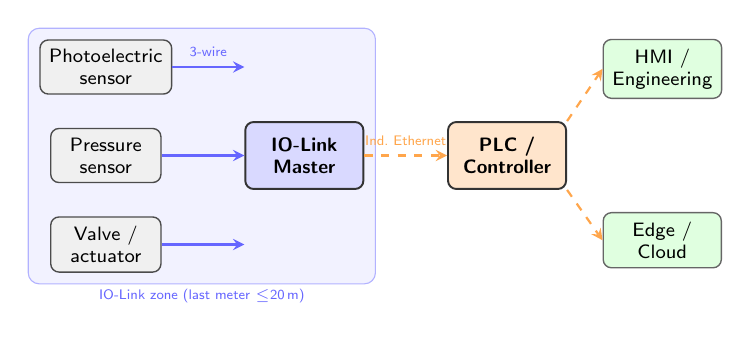
\begin{tikzpicture}[node distance=0.42cm and 0.48cm]

  % Field devices
  \node[device] (photo) {Photoelectric\\sensor};
  \node[device, below=of photo] (press) {Pressure\\sensor};
  \node[device, below=of press] (valve) {Valve /\\actuator};

  % IO-Link master
  \node[master, right=1.05cm of press] (master) {IO-Link\\Master};

  % PLC
  \node[controller, right=1.05cm of master] (plc) {PLC /\\Controller};

  % Upper systems
  \node[cloud, above right=0.28cm and 0.45cm of plc] (hmi)  {HMI /\\Engineering};
  \node[cloud, below right=0.28cm and 0.45cm of plc] (edge) {Edge /\\Cloud};

  % IO-Link arrows
  \draw[iolink] (photo.east) --
        node[above, font=\tiny\sffamily]{3-wire}
        (master.west |- photo.east);
  \draw[iolink] (press.east) -- (master.west);
  \draw[iolink] (valve.east) -- (master.west |- valve.east);

  % Industrial Ethernet arrow
  \draw[ethernet] (master.east) --
        node[above, font=\tiny\sffamily]{Ind.\ Ethernet}
        (plc.west);

  % PLC to upper systems
  \draw[ethernet] (plc.north east) -- (hmi.west);
  \draw[ethernet] (plc.south east) -- (edge.west);

  % Zone highlight
  \begin{scope}[on background layer]
    \node[draw=blue!30, fill=blue!5, rounded corners=4pt,
          fit=(photo)(press)(valve)(master),
          inner sep=4pt,
          label={[font=\tiny\sffamily\color{blue!60},yshift=2pt]
                 below:IO-Link zone (last meter $\leq$20\,m)}] {};
  \end{scope}

\end{tikzpicture}
\caption{Position of IO-Link in an automation system. Each port is a
dedicated point-to-point link; the master bridges field devices to the
Industrial Ethernet controller network.}
\label{fig:arch}
\end{figure}
% ──────────────────────────────────────────────────────────────────────────

The physical connection uses three wires: L$+$ and L$-$ for power, and
C/Q for the signal. The C/Q line carries either a conventional switching
signal in SIO mode or serial IO-Link communication. Standard M8 or M12
connectors support unshielded cables up to 20\,m. Port Class~A covers
most sensors; Port Class~B adds a separate auxiliary supply for
actuators with higher power demand~\cite{iols_sysdesc}.

The 20\,m cable limit is the most important placement constraint. In a
compact machine this is rarely a problem, but in larger plants masters
must be distributed. A useful feature is backward compatibility: a
master port can be configured as IO-Link, digital input, or digital
output, enabling gradual migration from conventional wiring.

\subsection{Communication and Data Types}

The master always initiates communication; devices only respond. Three
data rates are defined: COM1 at 4.8\,kbit/s, COM2 at 38.4\,kbit/s, and
COM3 at 230.4\,kbit/s. Each device supports one rate; a conforming
master detects it automatically.

The protocol separates data into four types:
\begin{itemize}
  \item \textbf{Process data} --- exchanged cyclically, up to
        32~octets per direction per cycle.
  \item \textbf{Value status} --- indicates whether the current cyclic
        data are valid.
  \item \textbf{Device data} --- read or written acyclically by index
        and subindex; covers identity, parameters, and commands.
  \item \textbf{Events} --- report errors and maintenance conditions
        such as wire break, contamination, or overtemperature.
\end{itemize}

The cyclic and acyclic channels operate in parallel: a PLC receives
measurements every cycle while an engineering tool reads diagnostics in
the background without interruption. Error detection uses a checksum on
every frame; if a frame fails, the master retries up to twice before
reporting a fault~\cite{iols_sysdesc}.

End-to-end latency depends on the device minimum cycle time, data
length, communication rate, master processing, fieldbus update, and PLC
scan. These must be summed and verified for each installation.

\subsection{IODD, Parameterization, and Diagnostics}

Every conforming IO-Link device ships with an IO Device Description
(IODD) file~\cite{iol_iodd}: a machine-readable XML file describing
communication properties, identity, process-data structure, parameters,
and diagnostic events. Engineering software imports the IODD and
presents device settings in a consistent interface across manufacturers.

Parameter data storage lets the master save all device parameters and
restore them automatically when a compatible replacement is connected.
The diagnostic channel provides specific fault information---contaminated
optics, overtemperature, low supply voltage---rather than a generic
fault bit. These diagnostics only reduce downtime when the control
program and maintenance team actively use them.

%% ---------------------------------------------------------------
\section{Application Scenario and Evaluation}
\label{sec:scenario}
%% ---------------------------------------------------------------

\subsection{Automated Packaging and Sorting Cell}

The evaluation scenario is a small packaging cell in which bottles move
on a conveyor, are checked, and are directed to an accepted or rejected
path. The devices are: a photoelectric sensor for bottle detection, a
distance sensor to check fill level, a pressure sensor for the
pneumatic supply, and a valve actuator for the sorting gate. All
connect to an eight-port IO-Link master over PROFINET to the PLC, with
an HMI for process display and diagnostics.

Figure~\ref{fig:infoflow} shows the information flow. Cyclic process
data travel from sensors to the PLC continuously. The PLC makes the
sorting decision and drives the gate. Recipe parameters and diagnostics
flow through the acyclic channel to and from the HMI.

% ── Figure 2: Information flow ─────────────────────────────────────────────
\begin{figure}[!t]
\centering
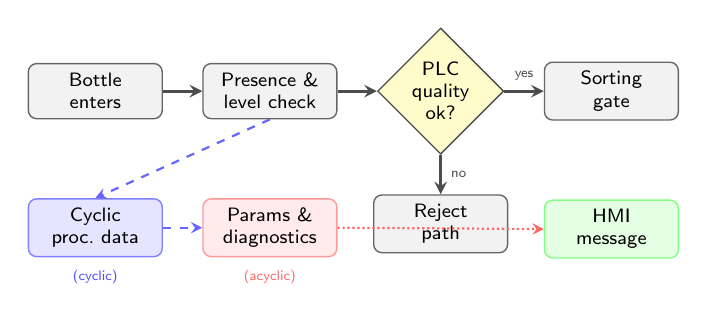
\begin{tikzpicture}[node distance=0.48cm and 0.5cm]

  % Physical process row
  \node[procbox] (bottle) {Bottle\\enters};
  \node[procbox, right=of bottle] (check)  {Presence \&\\level check};
  \node[decision, right=of check]  (dec)   {PLC\\quality\\ok?};
  \node[procbox, right=of dec]    (gate)   {Sorting\\gate};

  % Physical flow
  \draw[flow] (bottle) -- (check);
  \draw[flow] (check)  -- (dec);
  \draw[flow] (dec)    -- node[above,font=\tiny\sffamily]{yes} (gate);

  % Reject branch
  \node[procbox, below=0.5cm of dec] (reject) {Reject\\path};
  \draw[flow] (dec.south) -- node[right,font=\tiny\sffamily]{no} (reject.north);

  % Data channel row
  \node[procbox, fill=blue!10, draw=blue!50,
        below=1.0cm of bottle] (cyclic)
        {Cyclic\\proc.\ data};

  \node[procbox, fill=red!8, draw=red!40,
        below=1.0cm of check] (acyclic)
        {Params \&\\diagnostics};

  \node[procbox, fill=green!10, draw=green!50,
        below=1.0cm of gate] (hmi)
        {HMI\\message};

  % Data arrows
  \draw[dataflow] (check.south) -- (cyclic.north);
  \draw[dataflow] (cyclic.east) -- (acyclic.west);
  \draw[acyclic]  (acyclic.east) -- (hmi.west);

  % Channel labels
  \node[font=\tiny\sffamily\color{blue!70},
        below=0.04cm of cyclic]  {(cyclic)};
  \node[font=\tiny\sffamily\color{red!60},
        below=0.04cm of acyclic] {(acyclic)};

\end{tikzpicture}
\caption{Information flow in the packaging cell. Solid arrows show the
physical process; dashed and dotted arrows show the IO-Link cyclic and
acyclic data channels respectively.}
\label{fig:infoflow}
\end{figure}
% ──────────────────────────────────────────────────────────────────────────

\subsection{Communication Requirements}

Table~\ref{tab:req} defines the requirements used for evaluation. The
10\,ms update target is specific to this conveyor application.

\begin{table}[!t]
\caption{Requirements for the Packaging Cell}
\label{tab:req}
\renewcommand{\arraystretch}{1.25}
\begin{tabularx}{\columnwidth}{@{}p{0.5cm} p{3.15cm} p{3.05cm}@{}}
\toprule
\textbf{ID} & \textbf{Requirement} & \textbf{Evaluation criterion} \\
\midrule
R1 & Sensor values reach PLC within a 10\,ms application update target. &
     Device cycle, master, fieldbus, and PLC scan checked as a chain. \\[2pt]
R2 & Product thresholds changed from HMI without visiting each sensor. &
     Indexed parameter write via IODD engineering tool. \\[2pt]
R3 & Device faults show a meaningful cause on the HMI. &
     Value status, events, and device diagnostics. \\[2pt]
R4 & Replacement sensor recovers approved settings automatically. &
     Identity check and master data storage. \\[2pt]
R5 & Standard 24\,V wiring within 20\,m. &
     Three-wire connection and cable limit. \\[2pt]
R6 & Interface integrates into existing PROFINET system. &
     Master as fieldbus-independent gateway. \\[2pt]
R7 & Unauthorized parameter changes controlled. &
     Physical zone and PLC/master access control. \\
\bottomrule
\end{tabularx}
\end{table}

\subsection{Evaluation Method}

The evaluation is qualitative and requirements-driven. Each requirement
is mapped to protocol functions from the standard, noting where IO-Link
satisfies it fully, partially, or requires additional system-level
measures. Conventional 24\,V digital I/O and 4--20\,mA analog are used
as baselines. No measured latency is reported because no physical test
bench was available.

%% ---------------------------------------------------------------
\section{Evaluation and Discussion}
\label{sec:eval}
%% ---------------------------------------------------------------

\subsection{Performance and Requirement Fit}

\textbf{R1 -- Timing.}
IO-Link provides master-controlled cyclic communication, but meeting
the 10\,ms target is not automatic. The full end-to-end timing chain
must be summed:

\begin{equation}
t_\text{total} \approx t_\text{dev} + t_\text{master} +
                        t_\text{fieldbus} + t_\text{PLC}
\label{eq:timing}
\end{equation}

As a rough estimate for this cell: a COM2 device with a 2\,ms minimum
cycle, 2\,ms master processing, 4\,ms PROFINET update, and 2\,ms PLC
scan gives approximately 10\,ms end-to-end --- exactly at the target
with no margin. A COM1 device or a longer PLC scan would exceed it.
The designer must verify each element during commissioning.

Raw bandwidth is intentionally modest. COM3 at 230.4\,kbit/s is far
below Industrial Ethernet, but sensor messages are small. Up to
32\,octets per cycle per device is sufficient for measurements, status
bits, and actuator commands.

\textbf{R2, R3, R4 -- Smart device functions.}
These three requirements are where IO-Link provides the clearest
benefit. Remote parameter access via the IODD allows an HMI or PLC to
load a product recipe without visiting the sensor. Diagnostic events
identify the specific fault cause rather than a generic error bit.
Parameter data storage means a replacement device is configured
automatically. Together these functions reduce changeover time, shorten
mean time to repair, and lower configuration error risk.

\textbf{R5, R6 -- Wiring and integration.}
The three-wire 24\,V connection uses familiar field wiring. PROFINET
integration is handled by the master as a transparent gateway. The
20\,m limit suits a compact cell; in a larger plant, masters must be
distributed closer to devices.

\textbf{R7 -- Security.}
Only partly covered by the base protocol. The point-to-point topology
limits network exposure, but the protocol provides no encryption,
authentication, or access control~\cite{iol_security}. Parameter
changes must be protected through PLC user management, master access
control, and a secured engineering network.

\subsection{Comparison with Conventional Interfaces}

Table~\ref{tab:compare} summarizes the main trade-offs. Conventional
solutions remain appropriate in many cases. A digital input is simpler
and cheaper for a fixed limit switch. A 4--20\,mA loop handles long
distances and resists electrical noise. IO-Link is the better choice
when additional device information saves real time during commissioning,
changeovers, or fault diagnosis.

\begin{table}[!t]
\caption{Comparison of Field-Device Interfaces}
\label{tab:compare}
\renewcommand{\arraystretch}{1.2}
\begin{tabularx}{\columnwidth}{@{}p{1.45cm} p{1.6cm} p{1.55cm} p{1.9cm}@{}}
\toprule
\textbf{Criterion} & \textbf{Digital I/O} & \textbf{4--20\,mA} & \textbf{IO-Link} \\
\midrule
Information  & One on/off state   & One process value  & Values, status, params, events \\[2pt]
Direction    & One-way            & Device to ctrl     & Bidirectional \\[2pt]
Parameters   & Local only         & Local only         & Remote via IODD \\[2pt]
Diagnostics  & Wire state         & Limited            & Standardized events \\[2pt]
Replacement  & Manual             & Manual             & Auto restore \\[2pt]
Cable        & 24\,V std          & Dedicated line     & 3-wire, $\leq$20\,m \\[2pt]
Cost         & Lowest             & Low                & Master adds cost \\[2pt]
Best fit     & Switches           & Long-distance      & Smart sensors, flex.\ machines \\
\bottomrule
\end{tabularx}
\end{table}

\subsection{Advantages and Limitations}

The main advantages are: richer field data without extra cables;
vendor-independent device descriptions; remote configuration; automatic
parameter backup; detailed diagnostics; backward-compatible ports; and
fieldbus-independent integration. These are most valuable in flexible
machines with frequent product changes or condition monitoring needs.

The limitations are equally real. Each device occupies one master port.
The 20\,m cable limits placement options. Bandwidth is designed for
sensors, not cameras or large data streams. The base protocol has no
safety or security functions. Most importantly: diagnostics that nobody
monitors provide no value. The benefits of IO-Link depend on the
surrounding software, processes, and people.

%% ---------------------------------------------------------------
\section{Practical Integration Notes}
\label{sec:integration}
%% ---------------------------------------------------------------

Based on the standard documentation and our evaluation, several points
are relevant for an engineer planning a similar installation.

\textbf{Planning.}
Obtain the IODD for every device and verify communication rate, cycle
time, process-data length, and diagnostic events before ordering.
Select Port Class~A for sensors and Class~B for actuators needing
separate power. Place the master within 20\,m of all its devices.

\textbf{PLC programming.}
Map cyclic data into clearly named structures. Always check the value
status bit before trusting a measurement. Keep parameter and diagnostic
access in the acyclic channel, separate from the fast control loop.
Translate device event codes into plain-language HMI messages.

\textbf{Parameter management.}
Separate recipe parameters from protected calibration or service
parameters. Read back a parameter after writing to confirm success.
Configure master data storage deliberately so it backs up an approved
configuration, not an accidental change.

\textbf{Security.}
Keep field cables inside a physically controlled zone. Use individual
accounts and role-based permissions for engineering access. Route
remote access through the plant security architecture.

Table~\ref{tab:validation} proposes commissioning checks for the cell.
These are not results we measured; they are tests to be performed
during commissioning to confirm the requirements in
Table~\ref{tab:req} are met.

\begin{table}[!t]
\caption{Proposed Commissioning Checks (Not Experimentally Verified)}
\label{tab:validation}
\renewcommand{\arraystretch}{1.2}
\begin{tabularx}{\columnwidth}{@{}p{0.45cm} p{2.95cm} p{3.2cm}@{}}
\toprule
\textbf{T} & \textbf{Procedure} & \textbf{Expected result} \\
\midrule
T1 & Timestamp sensor change at PLC under load. &
     Worst-case update meets 10\,ms target. \\[2pt]
T2 & Load product recipe; read parameters back. &
     Values match recipe; invalid write gives clear fault. \\[2pt]
T3 & Replace sensor with compatible spare. &
     Master restores settings without local adjustment. \\[2pt]
T4 & Disconnect cable; trigger device warning. &
     HMI distinguishes comm.\ loss from device fault. \\[2pt]
T5 & Attempt parameter change as unauthorized user. &
     Change blocked; physical access restricted. \\
\bottomrule
\end{tabularx}
\end{table}

%% ---------------------------------------------------------------
\section{Selection Guidance and Limitations}
\label{sec:guidance}
%% ---------------------------------------------------------------

IO-Link should be chosen based on whether its functions solve a real
problem, not because it is newer technology. A fixed binary sensor
installed once and rarely changed does not justify a master port. In
contrast, an adjustable distance sensor used across multiple product
variants benefits directly from remote thresholds, contamination
warnings, and automatic parameter recovery.

A practical selection follows three steps: (1)~check the control
requirement: signal type, update deadline, safety relevance, and cable
distance; (2)~consider lifecycle needs: product changes, diagnostics,
replacement frequency, and maintenance skill; (3)~check system
constraints: master ports, fieldbus compatibility, IODD availability,
and engineering tool support. Table~\ref{tab:select} summarizes the key
decision questions.

\begin{table}[!t]
\caption{Technology Selection Questions}
\label{tab:select}
\renewcommand{\arraystretch}{1.2}
\begin{tabularx}{\columnwidth}{@{}p{3.45cm} p{3.7cm}@{}}
\toprule
\textbf{Question} & \textbf{Design consequence} \\
\midrule
Only one fixed on/off state? &
  Prefer digital I/O unless diagnostics add clear value. \\[2pt]
Long-distance continuous signal? &
  Consider 4--20\,mA; check 20\,m IO-Link limit. \\[2pt]
Thresholds change regularly? &
  IO-Link parameterization reduces manual setup. \\[2pt]
Detailed fault info needed? &
  Verify IODD includes the required events. \\[2pt]
Fast replacement by general staff? &
  Use identity checking and tested data-storage settings. \\[2pt]
Safety-critical or remotely exposed? &
  Apply full safety and security architecture above IO-Link. \\
\bottomrule
\end{tabularx}
\end{table}

This study has several limitations. The evaluation is based on standard
documents and a representative example, not laboratory measurements.
The timing estimate in~(\ref{eq:timing}) uses typical values for
illustration; actual values depend on the specific devices, master,
fieldbus, and PLC task configuration. The paper covers only wired base
IO-Link; IO-Link Safety, IO-Link Wireless, and cloud integration each
require separate study.

%% ---------------------------------------------------------------
\section{Conclusion}
\label{sec:conclusion}
%% ---------------------------------------------------------------

This paper examined wired IO-Link as the last-meter interface between
intelligent sensors and actuators and an industrial PLC. The standard
combines a 24\,V point-to-point connection with cyclic process data,
acyclic parameter access, standardized device descriptions, diagnostic
events, and parameter backup. For the packaging cell, these functions
address the main requirements: predictable sensor updates, remote
recipe change, meaningful diagnostics, automatic device replacement,
and PROFINET integration.

IO-Link is not always the right choice. Conventional digital or analog
I/O is simpler, cheaper, and sufficient for signals that never need
remote configuration or detailed diagnostics. The strongest case
appears when repeated changeovers, troubleshooting, or device
replacement would otherwise cause production downtime. Timing, cable
distance, security, and cost constraints must all be part of the design
decision.

Future work could implement the described cell and measure actual
end-to-end update time, retry behavior, and replacement time with a
specific master and device. A comparison with IO-Link Wireless would
also be valuable for applications where cable routing to each sensor is
impractical.

%% ---------------------------------------------------------------
\begin{thebibliography}{9}

\bibitem{iec61131}
International Electrotechnical Commission, ``IEC~61131-9:2022,
Programmable Controllers -- Part~9: Single-Drop Digital Communication
Interface for Small Sensors and Actuators (SDCI),'' 2022, edition~2.0.

\bibitem{iols_spec}
IO-Link Community, ``IO-Link Interface and System Specification,''
Version~1.1.4, Order No.~10.002, Jun.~2024. [Online]. Available:
\url{https://io-link.com/fileadmin/user_upload/Downloads/Package_2024/IOL-Interface-Spec_10002_V114_Jun24.pdf}

\bibitem{iols_sysdesc}
IO-Link Community, ``IO-Link System Description: Technology and
Application,'' 2018. [Online]. Available:
\url{https://io-link.com/fileadmin/user_upload/Downloads/About_IO-Link/IO-Link_System_Description_eng_2018.pdf}

\bibitem{galloway2013}
B.~Galloway and G.~P.~Hancke, ``Intro.\ to industrial control
networks,'' \textit{IEEE Commun.\ Surveys Tuts.},
vol.~15, no.~2, pp.~860--880, 2013.

\bibitem{moyne2007}
J.~R.~Moyne and D.~M.~Tilbury, ``The emergence of industrial control
networks for manufacturing control, diagnostics, and safety data,''
\textit{Proceedings of the IEEE}, vol.~95, no.~1, pp.~29--47, 2007.

\bibitem{wollschlaeger2017}
M.~Wollschlaeger, T.~Sauter, and J.~Jasperneite, ``The future of
industrial communication: Automation networks in the era of the internet
of things and industry~4.0,'' \textit{IEEE Industrial Electronics
Magazine}, vol.~11, no.~1, pp.~17--27, 2017.

\bibitem{iol_security}
IO-Link Community, ``IO-Link Secure Deployment Guideline,''
Version~1.0.0, Order No.~10.502, Jun.~2025. [Online]. Available:
\url{https://io-link.com/fileadmin/user_upload/Downloads/Security_Guidelines/IO-Link-SecureDeploymentGuideline_10502_V100_Jun25.pdf}

\bibitem{iol_iodd}
IO-Link Community, ``IO Device Description Specification,''
Version~1.1.4, 2024. [Online]. Available:
\url{https://io-link.com/downloads}

\bibitem{heynicke2018}
R.~Heynicke \textit{et al.}, ``IO-Link wireless enhanced factory
automation communication for industry~4.0 applications,'' \textit{Journal
of Sensors and Sensor Systems}, vol.~7, pp.~131--142, 2018.

\end{thebibliography}

\end{document}